%%%%%%%%%%%%%%%%%%%%%%%%%%%%%%%%%%%%%%%%%%%%%%%%%%%%%%%%%%%%%%%%%%%%%%%%%%%%%%%
%                       CARREGA DE LA CLASSE DE DOCUMENT                      %
%                                                                             %
% Les opcions admissibles son:                                                %
%      12pt / 11pt            (cos dels tipus de lletra; no feu servir 10pt)  %
%                                                                             %
% catalan/spanish/english     (llengua principal del treball)                 %
%                                                                             % 
% french/italian/german...    (si necessiteu fer servir alguna altra llengua) %
%                                                                             %
% listoffigures               (El document inclou un Index de figures)        %
% listoftables                (El document inclou un Index de taules)         %
% listofquadres               (El document inclou un Index de quadres)        %
% listofalgorithms            (El document inclou un Index d'algorismes)      %
%                                                                             %
%%%%%%%%%%%%%%%%%%%%%%%%%%%%%%%%%%%%%%%%%%%%%%%%%%%%%%%%%%%%%%%%%%%%%%%%%%%%%%%

\documentclass[11pt,spanish,listoffigures,listoftables]{tfgetsinf}
\bibliography{referencias}

%%%%%%%%%%%%%%%%%%%%%%%%%%%%%%%%%%%%%%%%%%%%%%%%%%%%%%%%%%%%%%%%%%%%%%%%%%%%%%%
%                     CODIFICACIO DEL FITXER FONT                             %
%                                                                             %
%    windows fa servir normalment 'ansinew'                                   %
%    amb linux es possible que siga 'latin1' o 'latin9'                       %
%    Pero el mes recomanable es fer servir utf8 (unicode 8)                   %
%                                          (si el vostre editor ho permet)    % 
%%%%%%%%%%%%%%%%%%%%%%%%%%%%%%%%%%%%%%%%%%%%%%%%%%%%%%%%%%%%%%%%%%%%%%%%%%%%%%%

\usepackage[utf8]{inputenc} 
\usepackage{listings}
\usepackage{tabularx,ragged2e,booktabs,caption}
\usepackage{makecell}
\usepackage{eurosym}
\usepackage{subfig}
%%%%%%%%%%%%%%%%%%%%%%%%%%%%%%%%%%%%%%%%%%%%%%%%%%%%%%%%%%%%%%%%%%%%%%%%%%%%%%%
%                        ALTRES PAQUETS I DEFINICIONS                         %
%                                                                             %
% Carregueu aci els paquets que necessiteu i declareu les comandes i entorns  %
%                                          (aquesta seccio pot ser buida)     %
%%%%%%%%%%%%%%%%%%%%%%%%%%%%%%%%%%%%%%%%%%%%%%%%%%%%%%%%%%%%%%%%%%%%%%%%%%%%%%%



%%%%%%%%%%%%%%%%%%%%%%%%%%%%%%%%%%%%%%%%%%%%%%%%%%%%%%%%%%%%%%%%%%%%%%%%%%%%%%%
%                        DADES DEL TREBALL                                    %
%                                                                             %
% titol, alumne, tutor i curs academic                                        %
%%%%%%%%%%%%%%%%%%%%%%%%%%%%%%%%%%%%%%%%%%%%%%%%%%%%%%%%%%%%%%%%%%%%%%%%%%%%%%%

\title{Implementación de sensores geolocalizados y una aplicación para la obtención de datos en un área metropolitana}
\author{\textbf{David Rodriguez Martinez}}
\tutor{\textbf{David Cuesta Frau}}
\curs{\textbf{2015-2016}}

%%%%%%%%%%%%%%%%%%%%%%%%%%%%%%%%%%%%%%%%%%%%%%%%%%%%%%%%%%%%%%%%%%%%%%%%%%%%%%%
%                     PARAULES CLAU/PALABRAS CLAVE/KEY WORDS                  %
%                                                                             %
% Independentment de la llengua del treball, s'hi han d'incloure              %
% les paraules clau i el resum en els tres idiomes                            %
%%%%%%%%%%%%%%%%%%%%%%%%%%%%%%%%%%%%%%%%%%%%%%%%%%%%%%%%%%%%%%%%%%%%%%%%%%%%%%%

\keywords{Ciutat Inteligent, Arduino, Hardware, Geolocalizació, Sensors, Harware lliure, Electrònica, Servicis Web} % Paraules clau 
         {Ciudad Inteligente, Arduino, Hardware, Geolocalizacion, Sensores, Harware Libre, Electronica, Servicios Web}              % Palabras clave
         {Arduino, Smart City, IoT, Remote Sensor, Open-source hardware}        % Key words
         
         %Arduino, Hardware Libre, Sensores, Control Remoto, Servidor Web, Electrónica, Arduino Shield, GPS.

%%%%%%%%%%%%%%%%%%%%%%%%%%%%%%%%%%%%%%%%%%%%%%%%%%%%%%%%%%%%%%%%%%%%%%%%%%%%%%%
%                              INICI DEL DOCUMENT                             %
%%%%%%%%%%%%%%%%%%%%%%%%%%%%%%%%%%%%%%%%%%%%%%%%%%%%%%%%%%%%%%%%%%%%%%%%%%%%%%%

\begin{document}

%%%%%%%%%%%%%%%%%%%%%%%%%%%%%%%%%%%%%%%%%%%%%%%%%%%%%%%%%%%%%%%%%%%%%%%%%%%%%%%
%              RESUMS DEL TFG EN VALENCIA, CASTELLA I ANGLES                  %
%%%%%%%%%%%%%%%%%%%%%%%%%%%%%%%%%%%%%%%%%%%%%%%%%%%%%%%%%%%%%%%%%%%%%%%%%%%%%%%


\begin{abstract}[spanish]
	
	El motivo de este proyecto es utilizar una plataforma de “hardware libre” llamada Arduino con el fin de implementar uno o varios nodos de sensores el cual enviará a través de la red Información sobre un área específica, y podremos monitorizar la informacion gracias a una aplicacion web.
	
	Mi intención es que gracias a lo explicado en el párrafo anterior se pueda implementar una utilidad hardware y una Web para utilizar en una Smart City\\
	
	\end{abstract}
\begin{abstract}

	El motiu d'aquest projecte es utilitzar una plataforma de "hardware lliure" anomenada arduino amb l'intencio d'implementar u o varios nodes de sensors, el cual enviara utilitzant una xarxa, informacio sobre una área específica la cual podrem monitoritzar gracies a una aplicació web . 

	La meua intenció es que gracies a el que he explicat en el parraf anterior es puga implementar una utilitat de gestió per utilitzar en una Smart City\\


\end{abstract}
\begin{abstract}[english]
	The purpose of this project is use a special Open-source hardware platform called Arduino, with the intention of implement one or more nodes of sensors, which will send on the network, information about a specific area that we can monitoring, using a web service.
	
	My intention is that thanks to I've explained in the last paragraph, i will can implement a hardware and web application to track that information to use in the future in the Smart city.\\

	
\end{abstract}
\lstlistoflistings
%%%%%%%%%%%%%%%%%%%%%%%%%%%%%%%%%%%%%%%%%%%%%%%%%%%%%%%%%%%%%%%%%%%%%%%%%%%%%%%
%                              CONTINGUT DEL TREBALL                          %
%%%%%%%%%%%%%%%%%%%%%%%%%%%%%%%%%%%%%%%%%%%%%%%%%%%%%%%%%%%%%%%%%%%%%%%%%%%%%%%

\mainmatter

%%%%%%%%%%%%%%%%%%%%%%%%%%%%%%%%%%%%%%%%%%%%%%%%%%%%%%%%%%%%%%%%%%%%%%%%%%%%%%%
%                                  INTRODUCCIO                                %
%%%%%%%%%%%%%%%%%%%%%%%%%%%%%%%%%%%%%%%%%%%%%%%%%%%%%%%%%%%%%%%%%%%%%%%%%%%%%%%


\chapter{Introducción a la práctica}

Esta práctica de Lenguajes y entornos de programación paralela consiste en la explotación de la GPU con el fin de poder obtener unos resultados de ejecución de problemas pesados para poder ser comparados entre diversos dispositivos y modelos de ejecución a fin de saber cuánta mejora ofrece este sistema de procesamiento.

El cálculo acelerado es el uso de una unidad de procesamiento gráfico en combinación con una CPU para acelerar aplicaciones de empresa, ingeniería, análisis y cálculo científico.\\
Gracias a esto las GPU aceleradoras han pasado a instalarse en centros de datos energéticamente eficientes de laboratorios gubernamentales, universidades y grandes compañías de todo el mundo. Las GPUs aceleran las aplicaciones de plataformas diversas, desde automóviles hasta teléfonos móviles y tablets, drones y robots.

Para ello he realizado la práctica bajo \textit{OpenCL}, una serie de librerías aportadas por \textit{CUDA GPU Programming}.

Con esto implementaremos un código en C que incorpora este modelo de programacion paralela que se ejecutara numerosas veces mientras se le aumenta la talla del problema, además se compararán diversas tecnologías, como la explotación de un solo núcleo (programación secuencial), \textit{CUDA} y \textit{OpenCL} (programación paralela) a fin de obtener una serie de resultados en los que se aplicaran diferentes comparaciones y conclusiones.

Además OpenCL es una especificación desarrollada por Apple, asi que se realizara una prueba en un entorno que incorpora nativamente OpenCL (OS X) con el fin de ver cómo de sencillo resulta trabajar con esta especificación en un entorno preparado.


%\section{Notes bibliografiques} %%%%% Opcional

%????? ????????????? ????????????? ????????????? ????????????? ?????????????

%%%%%%%%%%%%%%%%%%%%%%%%%%%%%%%%%%%%%%%%%%%%%%%%%%%%%%%%%%%%%%%%%%%%%%%%%%%%%%%
%                         CAPITOLS (tants com calga)                          %
%%%%%%%%%%%%%%%%%%%%%%%%%%%%%%%%%%%%%%%%%%%%%%%%%%%%%%%%%%%%%%%%%%%%%%%%%%%%%%%


\chapter{Estudio del Arte}

\setlength{\parindent}{5ex}En este capitulo se hablara de porque se han elegido las tecnologías que se van a utilizar en el proyecto asi como mostrar algunas de las opciones adicionales que se podrían haber utilizado. 

\section{¿Porque Arduino?}

Arduino es una plataforma Hardware Open Source lo que implica que todo el sistema esta disponible a los usuarios y esto ayudara al proceso de montaje ya que una gran parte de personas (la comunidad de Arduino) trabajan de manera desinteresada en el desarrollo de librerías y aplicaciones para esta plataforma. 
\setlength{\parindent}{0ex}

Sin embargo Arduino dispone de numerosas versiones por lo que dentro de las mas famosas que hay he decidido analizar cual de los que hay me ofrece mas garantías a la hora de realizar el proyecto por lo que en principio me decantare por el consumo de las microcontroladora, puertos y conexiones disponibles y disponibilidad.

En primer lugar he realizado un estudio del consumo de las placas disponibles para poder realizar este proyecto, 

\begin{center}
	\begin{tabular}{c c c } 
		\hline
		\textbf{Board} & \textbf{Consumo(W/h)} & \textbf{Consumo(mA/h)} \\ [0.3ex] 
		\specialrule{.08em}{1em}{0em}
		Arduino UNO & 0.23 & 46  \\ 
		Arduino DUE & 0.375 & 75  \\
		Arduino MEGA & 0.465 & 93  \\
		Arduino Nano & 0.075 & 15  \\
		Raspberry Pi & 1.77 & 353  \\ [1ex] 
		\hline
	\end{tabular}
	\captionof{table}{Consumo de los diferentes dispositivos} \label{tab:table1} 
\end{center}

En este caso nos interesaría el elegir el dispositivo que menor consumo tenga pero también he tenido que mirar que funcionalidad pueden aportar cada placa, cabe destacar que la Raspberry Pi no es una microcontroladora, si no un ordenador de placa reducida, pero ofrece una funcionalidad que podría mejorar las prestaciones de este proyecto, hablando de seguridad y comunicación, pero sin embargo después de las pruebas de consumo comparando con el Arduino que mas consume, en este caso el MEGA, consume en mA un 379\% mas ya que necesita mantener un sistema operativo que aunque sigue siendo un consumo muy bajo para ser un ordenador, es muy elevado para este proyecto así que en este punto descartamos la Raspberry Pi.

Otro punto a tener en cuenta son las capacidades de conexión que tienen las microcontroladoras, ya que para poder conectarlo todo voy a necesitar 3 entradas analógicas, una  entrada digital, 2 entradas para el rx y tx del puerto serie y compatibilidad con la Shield ethernet de Arduino.

El Arduino UNO es una muy buena opción ya que tiene todo esto y es de un consumo reducido aun así, la comunicación serial va por software ya que hay que implementar una librería especial para poder realzar un puerto serie para comunicarse con el GPS, ademas habría que diseñar un circuito por los problemas en los voltajes de las lecturas digitales ya que algunos componentes devuelven 3.3V y Arduino los detecta a 5V, que bien que no daría problemas pero podría dar lugar a valores anómalos en determinadas ocasiones.

El Arduino MEGA es la mejor opción disponible sin embargo ajustando con el material disponible, he de elegir el Arduino DUE ya que tiene un consumo mas reducido.

Estas son las características del Arduino DUE:

\begin{itemize}
\item \textbf{Microcontrolador}: AT91SAM3X8E
\item \textbf{Velocidad de reloj:} 84 MHz
\item \underline{\textbf{Tensión de trabajo:} 3.3V}
\item \underline{\textbf{Pines de entradas digitales:} 54}
\item \underline{\textbf{Pines de entradas analógicas: }12}
\item \underline{\textbf{Memoria Flash:} 512 KB}
\end{itemize}

He subrayado los valores que son importantes ya que en el estudio del montaje en el Arduino UNO tenia problemas con la memoria del programa ya que la memoria Flash quedaba casi completa utilizando la librería que implementaba un serial en cualquier pin digital,  imposibilitando la capacidad de poder implementar mejoras en la aplicación.

\section{Presupuesto}

En esta parte del proyecto se va a realizar un estudio de lo que puede llegar a costar la creación, el montaje y el mantenimiento de la aplicación, todo ello al precio actual del año 2016.

Em primer lugar se expondrá el coste de que costaría aproximadamente cada nodo de la aplicación:

\begin{itemize}
	\item \textbf{Arduino DUE:} 36\euro 
	\item \textbf{Shield de Ethernet:} 26\euro 
	\item \textbf{Neo6Mv2:} 13,50\euro 
	\item \textbf{Sensor de Gas MQ-7:} 8\euro 
	\item \textbf{Sensor de Temperatura y Humedad DHT11:} 3\euro 
	\item \textbf{Sensor de Sonido:} 0,50\euro 
	\item \textbf{Sensor de Luz:} 1\euro 
\end{itemize}

Todo esto nos da un coste de \textbf{88 \euro} por nodo de sensores aproximadamente.

Se podrían utilizar materiales mas baratos con el fin de reducir los costes aun mas pero no seria aconsejable pues del proyecto interesa que este activo el mayor tiempo posible. También se pueden modificar los elementos del mismo, nombrados en la parte donde se realizaba el estudio del consumo de energía de cada controladora (\textbf{Tabla \ref{tab:table1}}) realizando las modificaciones necesarias para que este pueda funcionar.

También se ha incluido el coste de lo que costaría añadir el servidor de la aplicación, en este caso he puesto componentes genéricos:

\begin{itemize}
	\item \textbf{Servidor:} 600\euro 
	\item \textbf{Router:} 30\euro 
	\item \textbf{Cableado:} 12\euro 
\end{itemize}

Todo esto nos da un coste de \textbf{642 \euro} por servidor aproximadamente, pero, como se ha explicado antes, todo esto se puede reducir con material ya disponible, porque, "quien no tiene un ordenador hoy día?".

Y por ultimo el mantenimiento de lo que seria todo el montaje, ya es difícil hablar de un mantenimiento pues la aplicación pues aumentaría con cada nodo añadido, la ampliación del servidor en caso de haber demasiadas peticiones, el modo de alimentar los nodos que podría ser por microUSB, POE o baterías, diferentes Controladoras, todo esto nos daría un resultado muy variable, así que es muy complicado cuanto costaría mantener la aplicación.

\section{Gestión del proyecto}

Para este proyecto se va a gestionar el proyecto utilizando una aplicación Web llamada \textit{Bitbucket}:

\textit{Bitbucket es un servicio de alojamiento basado en web, para los proyectos que utilizan el sistema de control de revisiones Mercurial y Git.}\cite{bitbucket}.

En esta aplicación se irán subiendo todos los cambios que se realicen en este proyecto ya que ofrece una gestión bastante sencilla de los proyectos y las versiones de cada una, ademas cuenta con una aplicación llamada \textit{sourceTree} que permite conectar con una cuenta de \textit{Bitbucket} y permitirá realizar las subidas de ficheros desde el mismo sistema operativo sin tener que acceder desde el navegador y ademas gestionar de una manera sencilla todas las versiones del proyecto.

\begin{figure}[!h]
	\centering
	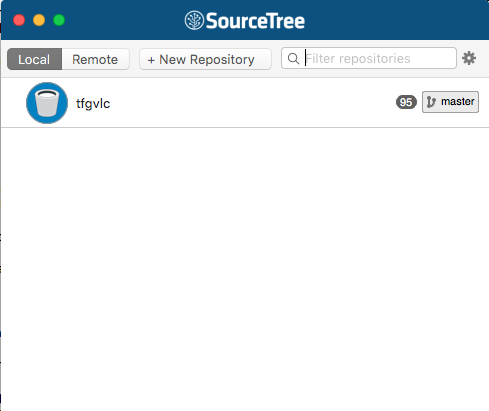
\includegraphics[width=0.3\linewidth]{figuras/stree}
	\caption{Gestion de proyectos con \textit{SourceTree}}
	\label{fig:stree}
\end{figure}

\chapter{Descripción del proyecto}

\setlength{\parindent}{5ex}Para este proyecto voy a utilizar una micro controladora Arduino DUE desatollada por \textbf{Arduino} , en esta se implementaran una serie de sensores y librerías que permitirán realizar una serie de funciones. Para enviar la información a la red, dicha controladora necesitara una Shield que le permita conectarse a la red también desatollada por \textbf{Arduino}.

\setlength{\parindent}{0ex}Para recoger toda esta información se diseñara una aplicación que reciba las peticiones y pueda almacenarlas en una base de datos, a su vez esta aplicación web también servirá esta información al usuario de una manera detallada para su estudio.

Finalmente se le ofrece al usuario generar unos reportes en los que este podrá descargarlos para, en un futuro, poder trabajar con esa información en otros programas o plataformas.

Esta es la explicación de las tecnologías y dispositivos que voy a utilizar:

\section{Tecnologías utilizadas}

\subsection{Arduino}

\setlength{\parindent}{5ex}\textbf{Arduino DUE }es una placa Microcontroladora basada en el Atmel SAM3X8E ARM Cortex-M3 CPU. Es el primer Arduino basado en un Núcleo microcontrolador ARM de 32 bits ya que su versión anterior (Arduino UNO), trabaja directamente sobre un microcontrolador.

\begin{figure}[!h]
	\centering
	
\includegraphics[width=0.2\linewidth]{figuras/ardulogo}
	\caption{Logo Arduino}
	\label{fig:ardulogo}
\end{figure}

\setlength{\parindent}{0ex}Para programar estas controladoras es necesario utilizar el IDE de Arduino, realizando una comunicación serie entre la maquina y la controladora podremos realizar un flash de la memoria con el fin de incorporar a la memoria interna del Arduino DUE el programa que hemos diseñado para realizar las funciones. 
Para programarlo se utiliza una versión simplificada de C++ la cual realiza una configuración inicial (Setup) y un bucle infinito (Loop), una vez arrancado el programa en la controladora este se repetirá indefinidamente realizando siempre la función programada. 

El IDE de Arduino podemos descargarlo de aquí:

\url{https://www.arduino.cc/en/Main/Software}

\subsection{GPS y Nmea Data}

Para el proyecto vamos a utilizar el GPS Neo6mv2, este GPS es bastante útil ya que es barato y de bajo consumo, ideal para la propuesta del proyecto ya que lo que se interesa es el ahorro de energia.

Este GPS nos podrá enviar información útil del satélite como la posición, la altitud, la fecha y la hora todo utilizando un formato de cadena Hexadecimal llamada NMEA DATA

\subsection{Nmea Data}

"\textit{El National Marine Electronics Association (NMEA) ha desarrollado una especificación que define la interfaz entre varias piezas de equipos electrónicos. La norma permite la electrónica de la  marina enviar información a los ordenadores ya otros equipos marinos.}"

Los receptores GPS están incluidos en esta especificación. Muchos de los programas de Posicionamiento están comprendidos bajo el formato NMEA. Estos datos incluyen PVT \textit{(Posición, Velocidad, Tiempo)} generada por el receptor GPS. La idea del NMEA es enviar información llamada frase la cual es totalmente independiente de otras frases.

\subsection{Formato del NMEA Data}

El modulo Neo6Mv2 funciona enviado al serie cadenas de números hexadecimales en formato de NMEA data. El GPS envía información al serie cada intervalo de tiempo por lo que no sería necesario el puerto Tx del Arduino ya que solo se va a recibir información, no obstante, lo he configurado con el fin de poder configurar lo desde el Arduino.

Este es el resultado que envía el GPS por el Serial2 del Arduino:

\begin{lstlisting}
$GPRMC,192128.00,V,,,,,,,150216,,,N*7D
$GPVTG,,,,,,,,,N*30
$GPGGA,192128.00,,,,,0,00,99.99,,,,,,*67
$GPGSA,A,1,,,,,,,,,,,,,99.99,99.99,99.99*30
$GPGSV,1,1,01,06,,,18*77
$GPGLL,,,,,192128.00,V,N*4B
\end{lstlisting}
Si analizamos los datos, siguiendo la especificación de la NMEA data averiguamos que funciona pero no correctamente pues este aun no esta devolviendo una localización.
Para ello el GPS tiene que estar en contacto directo con el satélite, por lo que hemos de ponerlo al aire libre, y una vez hecho esto este se conectará automáticamente dando este resultado:

\begin{lstlisting}
$GPRMC,192232.00,V,,,,,,,150216,,,N*75
$GPVTG,,,,,,,,,N*30
$GPGGA,192232.00,,,,,0,00,99.99,,,,,,*6F
$GPGSA,A,1,,,,,,,,,,,,,99.99,99.99,99.99*30
$GPGSV,2,1,06,02,35,106,52,06,28,058,48,12,69,064,46,19,11,045,49*7D
$GPGSV,2,2,06,21,,,35,24,40,151,4
\end{lstlisting}

\subsection{Laravel}

Basado en \textit{Symphony} Laravel es un framework Opensource que permite desarrollar aplicaciones y servicios web sirviéndose de una estructura Modelo-Vista-Controlador (MVC) ya creada en PHP 5.

Con este entorno desarrollare la aplicación web que nos servirá para almacenar  los datos y usara algunas tecnologías para ello.

\subsection{MySQL}

\setlength{\parindent}{5ex}MySQL es un SGBD (Sistema de Gestión de Bases de Datos)  relacional bajo licencia dual GPL por Oracle está considerada como la base datos open source más popular para entornos de desarrollo de aplicaciones Web.

\subsection{Bootstrap}

\textbf{Bootstrap} es una librería  CSS para el desarrollo de vistas para aplicaciones web. Utilizado para desarrollar la interfaz de usuario en paginas web, como los botones, formularios, cabeceras...

\subsection{Chart.js}

\textbf{Chart.js} es una librería JavaScript, utilizada para generar gráficos en el la vista de las aplicaciones web, es capaz de generar gráficos dinámicos, útil para el proyecto pues se implementara una serie de gráficos que monitorizaran la información obtenida.





\chapter{Montaje del Hardware y el Servicio Web}

\setlength{\parindent}{5ex}En este capitulo se va a explicar como se ha montado todo este sistema, así como una explicación de sus diferentes piezas y la función que realiza cada una de ellas tanto en la parte hardware como en la parte software.
También se realizara un estudio del coste de todos los materiales, así como el mantenimiento y consumo de estos.

\setlength{\parindent}{0ex}Esta es la estructura que se seguiremos para el montaje de la aplicación:

\begin{figure}[!h]
	\centering
	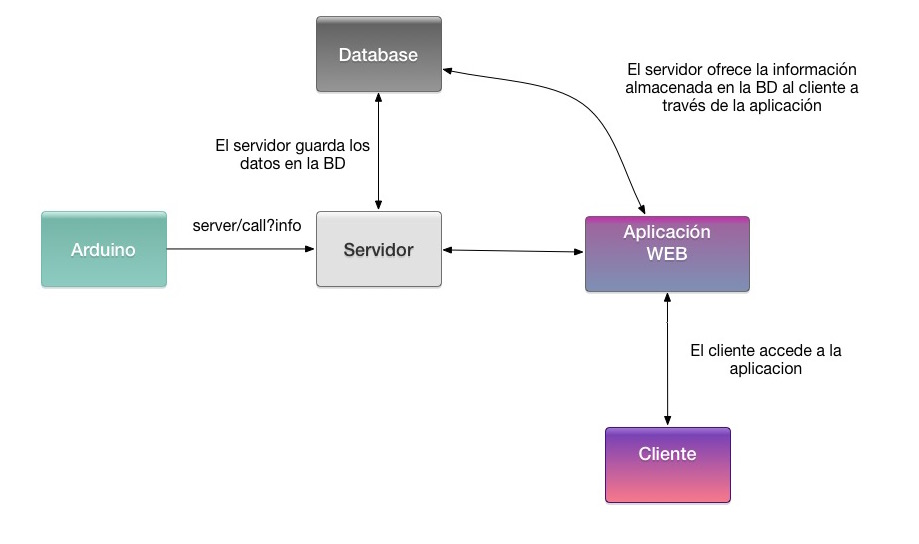
\includegraphics[width=0.9\linewidth]{figuras/montage1}
	\caption{Diagrama de montaje del proyecto en que función realizan las diferentes partes, desde el modulo hasta la información que podrá visualizar el cliente}
	\label{fig:imgmontage1}
\end{figure}



\section{Material}

\setlength{\parindent}{0ex}Para este proyecto se ha utilizado el siguiente material:\\

\textbf{Arduino Due:} Es la Controladora que se encarga de recibir la información y procesarla para enviarla al servidor.

\begin{figure}[!h]
	\centering
	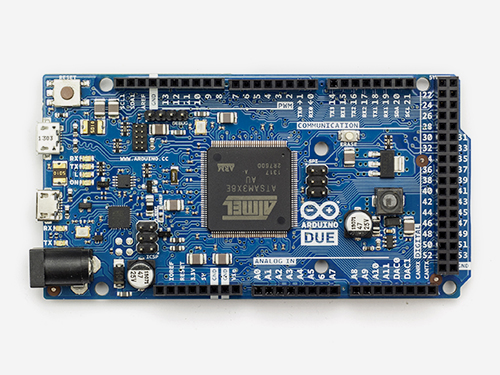
\includegraphics[width=0.4\linewidth]{figuras/arddue}
	\caption{Microcontroladora Arduino DUE}
	\label{fig:imgdue}
\end{figure}

\setlength{\parindent}{0ex}\textbf{Ethernet shield:} Es una Shield que permite a la micro controladora conectarse a la red.

\begin{figure}[!h]
	\centering
	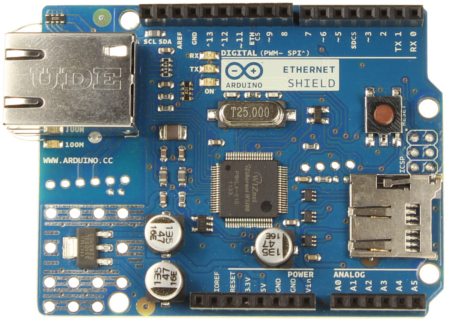
\includegraphics[width=0.3\linewidth]{figuras/ethshi}
	\caption{Ethernet shield}
	\label{fig:imgethshi}
\end{figure}

\setlength{\parindent}{0ex}\textbf{Modulo GPS NEO6mv2: }Es un módulo el cual contiene un GPS que una vez este conectado al satélite enviara información de la geolocalización.

\setlength{\parindent}{0ex}\textbf{Sensores:} Un conjunto de sensores que permitirá la obtención de los valores ambientales del entrono donde este instalado el nodo.

Estos sensores son:

\begin{itemize}
	\item \textbf{DHT11} Es el sensor de Humedad y temperatura de Adafruit recogerá estos datos climáticos.
	\item \textbf{Sensor de gas CO MQ-7 y el chipset LM393} el que se utilizara para la medición de gases en el ambiente.
	\item \textbf{Sensor luz y sonido} el cual también utiliza el chipset LM393 medirá la contaminación lumínica y acústica.
\end{itemize}

\textbf{Servidor:} El servidor que se va a utilizar para realizar las función de conexión entre el nodo y la la base de datos y entre el cliente y la conexión con el cliente a través de la aplicación web.

Las características de este servidor serán:

\begin{itemize}
	\item \textbf{CPU:} Intel i5 2500K a 3.3 GHz de funcionamiento.
	\item \textbf{Memoria:} 8 GB 1600 MHz DDR3.
	\item \textbf{Almacenamiento:} 2 TB de Almacenamiento, el que permitirá tener una base de datos bastante amplia.
	\item \textbf{S.O:} OSX El Capitan 10.11.6.
\end{itemize}

\textbf{Aplicaciones: } Aplicaciones que me han permitido realizar el montaje de todo el sistema.

Entre ellas están:

\begin{itemize}
	\item \textbf{Mamp:} Es una aplicación para montar un servidor web Apache y Mysql bajo los puertos 8888 para el web y 8889 para el Mysql.
	\item \textbf{MySQL Workbench} aunque es cierto que Laravel 5 gestiona la base de datos través de PHP se ha utilizado esta aplicación para poder gestionar la información almacenada en la base de datos.
	\item \textbf{PhpStorm } Un IDE de desarrollo para programar con PHP así como gestionar proyectos con Git.
\end{itemize}

\textbf{Cableado:} Distintos tipos de cableado para conectarlo todo.

\section{Montaje del Nodo Arduino DUE}

\setlength{\parindent}{5ex}El nodo para esta aplicación sera la microcontroladora con los módulos de sensores que enviaran información al servidor, para ello se realizara el montaje siguiendo el siguiente esquema:\\
\setlength{\parindent}{0ex}
\begin{figure}[!h]
	\centering
	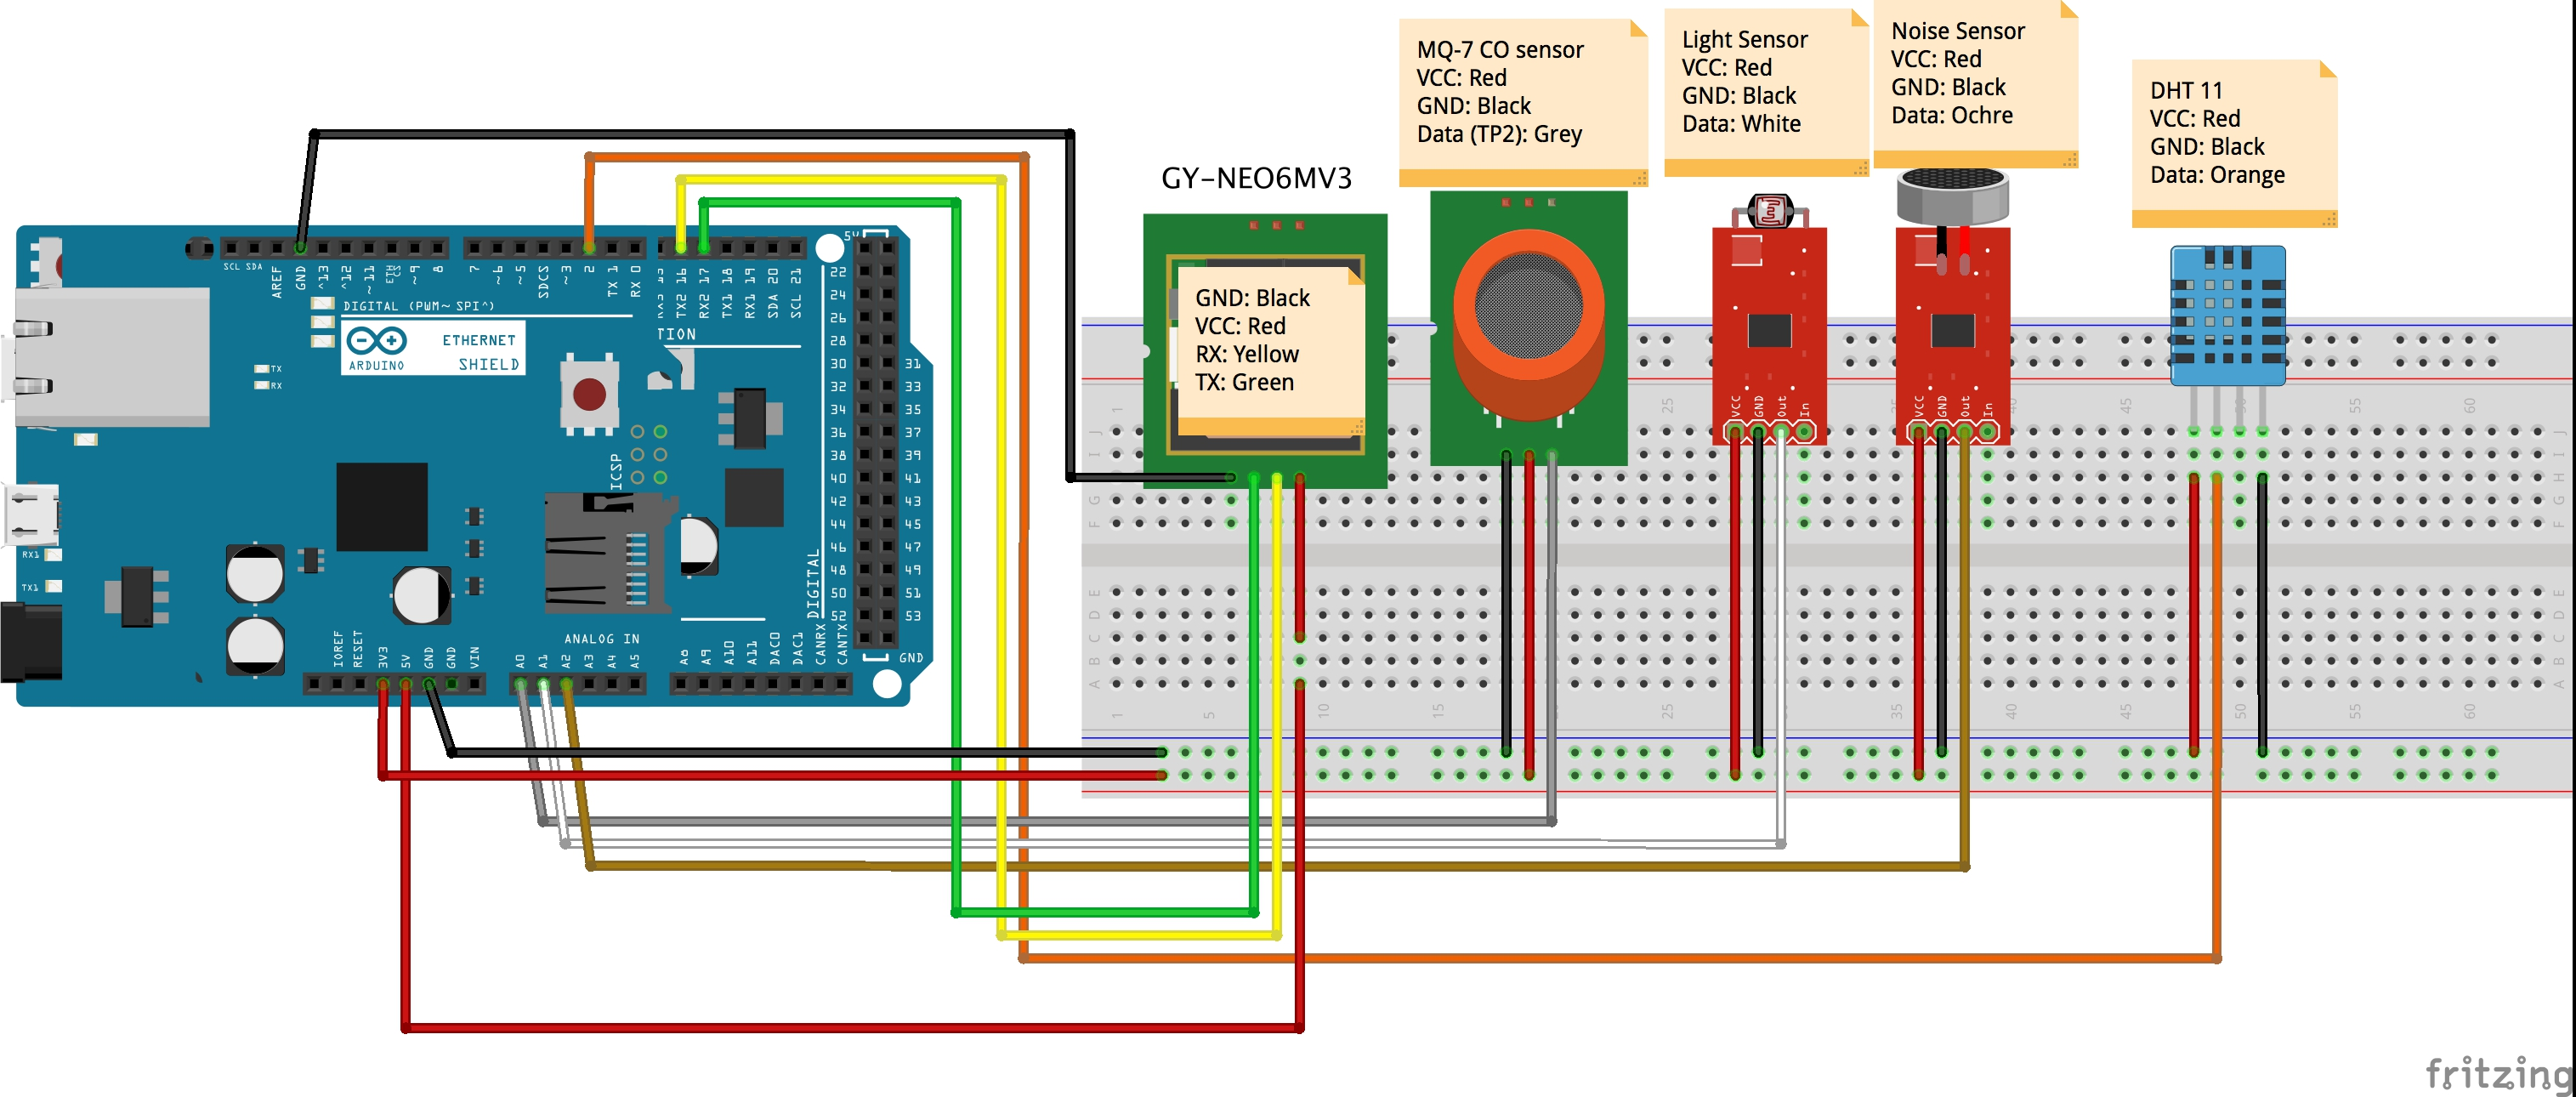
\includegraphics[width=0.9\linewidth]{figuras/ardschema}
	\caption{Esquema del montaje}
	\label{fig:imgdue}
\end{figure}

En la \textbf{Figura \ref{fig:imgdue}} se puede apreciar el esquema de las conexiones que he seguido para el montaje del nodo para que el código de la aplicación para Arduino recoja los valores correctamente.


Como se puede apreciar en el esquema el montaje es sencillo ya que no necesita electrónica adicional como resistencias u otros componentes electrónicos. Para conectar esto cada uno de los sensores, siguiendo el esquema, se conectara VCC (\textcolor{red}{Rojo}) a 3.3V ya que es el funcionamiento de cada uno de los sensores exceptuando el GPS que ira conectado a 5V ya que ha demostrado un mejor funcionamiento a ese voltaje y GND (\textcolor{black}{Negro}) para el negativo de los módulos, todos los sensores exceptuando el sensor de temperatura y humedad DHT11 que va a la entrada digital y el GPS que va conectado al Serial 2, van conectados a entradas analógicas (de A0 a A2).

Tener en cuenta que si se realiza en un Arduino UNO al ser una versión mas antigua las lecturas digitales se leen en un rango de 5V por lo que hay que diseñar un circuito especial para poder leer el GPS y el sensor DHT11 ya que estos devuelven una señal digital de 3.3V, para solucionar esto se tendrían que poner resistencias en el circuito con el fin de diseñar un sistema que aumente la señal a los 5V que necesita el Arduino UNO, que en este caso quedaría tal que así:

\begin{figure}[!h]
	\centering
	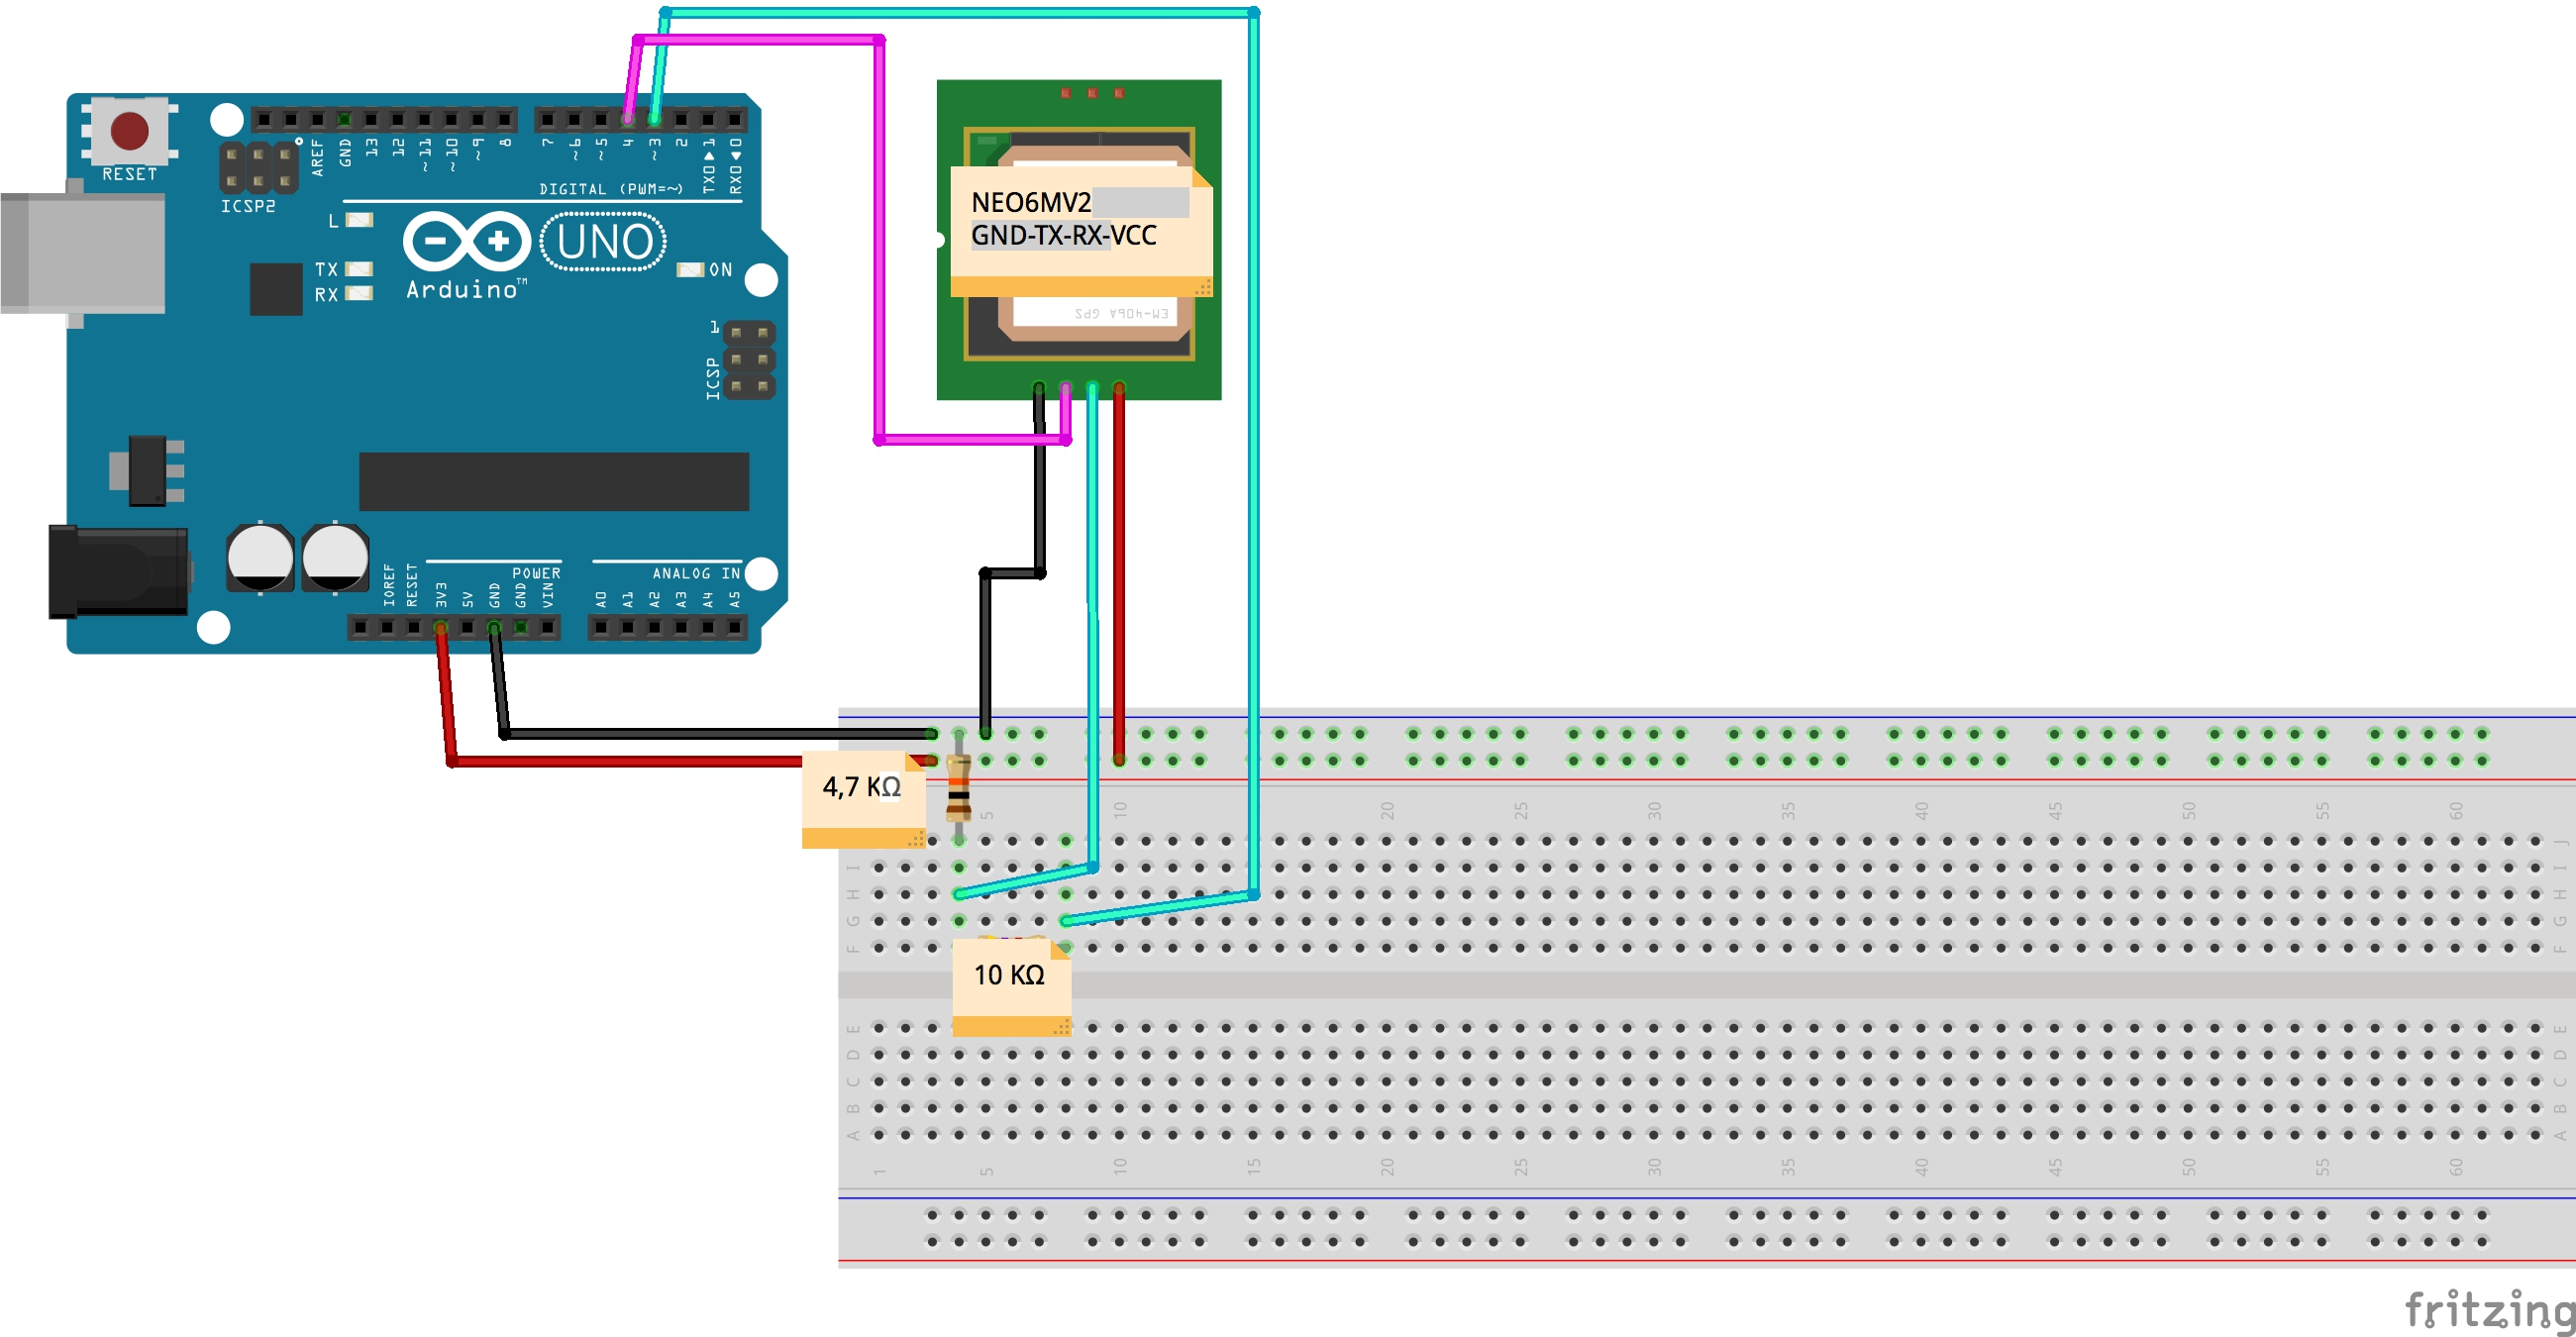
\includegraphics[width=0.9\linewidth]{figuras/unogps}
	\caption{Esquema del circuito para el GPS en el Arduino UNO}
	\label{fig:imgunogps}
\end{figure}

El circuito de la \textbf{Figura \ref{fig:imgunogps}} es un ejemplo de instalación para un modulo en Arduino UNO cuya respuesta en digital sea de 3.3V y sirve para otros módulos.

También comentar que los RX y TX de la trasmisión serie van conectados de manera invertida entre el GPS y el Arduino.

Cada uno de estos sensores tendrá su función en el código de manera modular, así que es mas sencillo entender el funcionamiento del mismo.

\section{Programación de la Microcontroladora Arduino DUE}

\setlength{\parindent}{5ex}En este apartado se va a explicar cada una de las partes del código que utilizara el Arduino DUE, dicha parte realizara una función en la controladora por lo que el conjunto de todo el código realizara la función propuesta para este proyecto.
\setlength{\parindent}{0ex}

El código se puede descargar de la siguiente URL: \url{https://bitbucket.org/Zhelix/tfg-vlc/downloads}\\

Esta es la parte de la configuración:

\begin{lstlisting}
/*
*  FILE:     project-v1.3.1.ino
*  AUTHOR:   David Rodriguez Martinez  davidrm146@gmail.com
*  VERSION:  1.3.1
*/
//Necessary Libraries
#include <Ethernet.h>
#include <SPI.h>
#include <TinyGPS.h>
#include "DHT.h"

//Config of the device
byte mac[] = { 0xDE, 0xAD, 0xBE, 0xEF, 0xFE, 0xED };
TinyGPS gps;
#define DHTPIN 2  
#define DHTTYPE DHT11  
DHT dht(DHTPIN, DHTTYPE);
IPAddress ip(192, 168, 1, 102);
EthernetClient client;
String data;
void setup()
{  
	Serial.println("EXECUTING setup");
	Serial.begin(9600);
	Serial2.begin(9600);
	if (Ethernet.begin(mac) == 0) {
		Serial.println("Failed to configure Ethernet using DHCP");
		Ethernet.begin(mac, ip);
	}
	delay(1000);   // A Small delay for avoid errors
}
\end{lstlisting}

Antes de entrar al código se implementaran las librerías para el funcionamiento de los módulos, en este caso lo que hacen es traducir la información para que pueda ser manipulada de manera mas fácil. las librerías son:

\begin{itemize}
	\item \#include <Ethernet.h>: Permite gestionar la conexión a la red.
	\item \#include <SPI.h>: Permite al Arduino DUE comunicarse con la Shield de Ethernet.
	\item \#include <TinyGPS.h> Esta librería traduce el NMEA data en valores legibles sin necesidad de manipular la cadena de hexadecimales recibida.
	\item \#include 'DHT.h':  Esta librería traduce la información recibida por el sensor DHT11, solo hace falta configurar que pin es el que recibirá la información y que tipo de sensor se va a utilizar ya que la librería configura automáticamente la comunicación con el sensor.
\end{itemize}

Esta es la configuración de Arduino encapsulada en la definición de SETUP en esta parte del código se definirá la comunicación vía serie para el modulo GPS conectado al serial 2 a 9600 baudios aunque aplicando una serie de cadenas hexadecimales en el arranque del programa escritas en el GPS vía serie.
También se configurara la conexión serie que le pertenece al puerto USB para poder observar la información que envía cada vez que se repita el bucle del programa con el fin de poder debugguearlo en caso de algún problema o fallo de los componentes.\\

\begin{lstlisting}
	if (Ethernet.begin(mac) == 0) {
		Serial.println("Failed to configure Ethernet using DHCP");
		Ethernet.begin(mac, ip);
	}
\end{lstlisting}
Esta parte es la conexión a la red, en este caso por DHCP que solo hace falta asignarle la MAC al dispositivo o si falla asignar manualmente una dirección IP que corresponderá a la dirección de la red interna.

Una vez configurado todo el programa ya estará listo para leer la información que recojan los módulos de sensores asi que se dieñara el siguiente codigo para realizar dicha lectura en la definición del LOOP el cual se ejecutara indefinidamente:\\

\begin{lstlisting}
void loop(){
	Serial.println("EXECUTING LOOP");
//***************GPS CODE*********************
	bool newData = false;
	unsigned long chars;
	unsigned short sentences, failed;
		for (unsigned long start = millis(); millis() - start < 1000;){
			while (Serial2.available()){
				char c = Serial2.read();
				if (gps.encode(c))newData = true;
			}
		}
	float flat, flon;
	unsigned long age;
	gps.f_get_position(&flat, &flon, &age);
	Serial.print("LAT=");
	Serial.print(flat == TinyGPS::GPS_INVALID_F_ANGLE ? 0.0 : flat, 6);
	Serial.print(" LON=");
	Serial.print(flon == TinyGPS::GPS_INVALID_F_ANGLE ? 0.0 : flon, 6);
	Serial.print(" SAT=");
	Serial.print(gps.satellites() == TinyGPS::GPS_INVALID_SATELLITES ? 0 : gps.satellites());
	Serial.print(" PREC=");
	Serial.println(gps.hdop() == TinyGPS::GPS_INVALID_HDOP ? 0 : gps.hdop());

//The next variable keeps the information collected by the sensors
	data = 
		"board_id=" +  getID()  +
		"&temp=" +  getTemperature()  + 
		"&hum=" + getHumidity() +
		"&gas="+ getGas() + 
		"&noise=" + getNoise() +
		"&luz="+ getLight() + 
		"&poslat=" + String(flat, 6) + 
		"&poslon=" + String(flon, 6);

//Debug function, this string works
//data ="board_id=1&temp=23&hum=43&gas=53&noise=54&luz=55&poslat=63&poslon=73";
		displayData(data);
//This function is for send information to the server
		sendDataGet(data);
delay(60000);
}
\end{lstlisting}

En esta parte del código se realizan 3 funciones, la lectura del GPS, el envío de la cadena que contiene las funciones que recogen de datos de los sensores y el delay que establecer un periodo de envío de información con el fin de evitar saturar la red.\\

\begin{lstlisting}
	for (unsigned long start = millis(); millis() - start < 1000;){
		while (Serial2.available()){
			char c = Serial2.read();
			if (gps.encode(c))newData = true;
		}
	}
\end{lstlisting}

Esto recogerá la información del gps en formato de NMEA data pero gracias a la librería TinyGPS.h que nos traduce directamente sin tener que editar manualmente el NMEA data, la información obtenida del GPS leyendo el Serial2 del Arduino DUE devolviendo nos información del GPS, en este caso nos interesa \textbf{flat} y \textbf{flon} que son las coordenadas que recoge el GPS.

 Los Serial.print están para mostrar la información obtenida ya que este no conecta al instante al satélite como ya se vera en el funcionamiento del vídeo mas adelante.

También se recoge la información para enviar al servidor en la variable \textbf{data} en la que se llaman las funciones que recogerán la información, es importante que el formato de la cadena sea como esta especificado en los comentarios, siguiendo el nombre de las variables ya que si no están bien nombrados la función del servidor que se encarga de recoger la información no funcionara y no se podrá realizar la inserción a la base de datos. Este es un ejemplo de como debería ser definida:\\

\begin{lstlisting}
		data="board_id={id} +
			&temp={temperatura} +
			&hum={humedad} +
			&gas={medicion del gas} +
			&noise={ruido ambiental} +
			&luz={luminosidad} +
			&poslat={latitud} +
			&poslon={longitud}";
\end{lstlisting}

Y por ultimo una delay o pausa que evitara que el Arduino esté enviando información constantemente de 1 minuto (60000 milisegundos)

Una vez explicado el bucle se explicaran las funciones que se ejecutan en la variable de datos ya que son las que recogen la información ambiental de la zona donde esta situado:\\

\begin{lstlisting}
String getTemperature() {
	float t = dht.readTemperature();
	float f = dht.readTemperature(true);
	if (isnan(t) || isnan(f)) {
		Serial.println("Failed to read Temperature from DHT. . .");
		return "0";
	}
	return String(t, 2);
}

String getHumidity() {
	float h = dht.readHumidity();
	if (isnan(h)) {
		Serial.println("Failed to read Humidity from DHT. . .");
		return "0";
	}
	return String(h, 2);
}

String getGas() {return String(analogRead(A0));}

String getLight() {	return String(analogRead(A1));}

String getNoise() {	return String(analogRead(A2));}

String getID() {return "1";}
\end{lstlisting}

En las funciones \textit{getTemperature} y \textit{getHumidity} se puede apreciar que gracias a la librería dht.h se realiza la conexión y lectura de la información del sensor sin tener que crear código adicional para controlar este sensor. Sobre las demás funciones son lecturas analógicas de las mismas que nos dan unos valores normales en su rango de 1 a 1024. Y la ultima sirve para establecer la id en la que esta registrada en la base de datos, este numero debe coincidir con su controladora como ya se explicará mas adelante.

Una vez ya esta explicado el código se explicara la llamada a la web la cual realizara la inserción a la bd, este es su código:

\begin{lstlisting}
void sendDataGet(String data) {
	if (client.connect("192.168.1.16",8888)){
		client.print("GET /call?");
		client.println(data);
		client.println("HTTP/1.1");
		client.println("Host: 192.168.1.16");        
		client.println("Connection: close");
		client.println();
	}
	if (client.connected()) { 
		client.stop();
	}
}
\end{lstlisting}

Esta función realiza la petición GET al servidor web el cual se configurara con la ip y el puerto en el que esté trabajando el servidor, puede ser publica o privada por lo que el Arduino puede trabajar en Internet aunque es mucho mas inseguro para la aplicación pues uno de sus puntos débiles es que el Arduino no tiene capacidad para la encriptación y tampoco tiene soporte para peticiones HTTPS por lo que una gran falla de este proyecto son los ataques \textit{man in the middle}, la llamada corresponde a una petición a la web "call?información..." en la cual se obtendrá la información en forma de JSON y sera almacenada den la BD.

La llamada o dirección del servidor web quedaría algo tal que así: 

\begin{lstlisting}
	192.168.1.16:8888/call?board_id={id}&temp={temperatura}&hum={humedad}&gas={medicion del gas}&noise={ruido ambiental}&luz={luminosidad}&poslat={latitud}&poslon={longitud}
\end{lstlisting}

Este es el código de la pagina web PHP que recogerá los datos en formato JSON y los guardara en la base de datos, todo ello realizado en Laravel 5.

\begin{lstlisting}
 public function setData(){
		 $getData = Request::all();
		 data::create($getData);
		 if (!$this->active){$this->setWorking(Request::get('board_id'));}
		 return $getData;
 }
\end{lstlisting}

La función \textit{\$getData = Request::all();} recoge toda la información que reciba en un GET o POST y lo introduce en la variable en formato JSON luego se ejecutaría el controlador de data la función \textit{data::create(\$getData);} de ahí la importancia que las variables introducidas en la variable data de Arduino estén nombradas como se ha especificado ya que en la BD se han de nombrar igual para que las entradas puedan ser introducidas correctamente.

Una vez configurado esto ya se podría dejar la microcontroladora trabajando para la recolección de datos.


\chapter{Explicación de la aplicación}

En este capitulo se explicara como funciona la aplicación WEB diseñada para recoger y mostrar los datos de cada uno de los sensores.

\begin{figure}[!h]
	\centering
	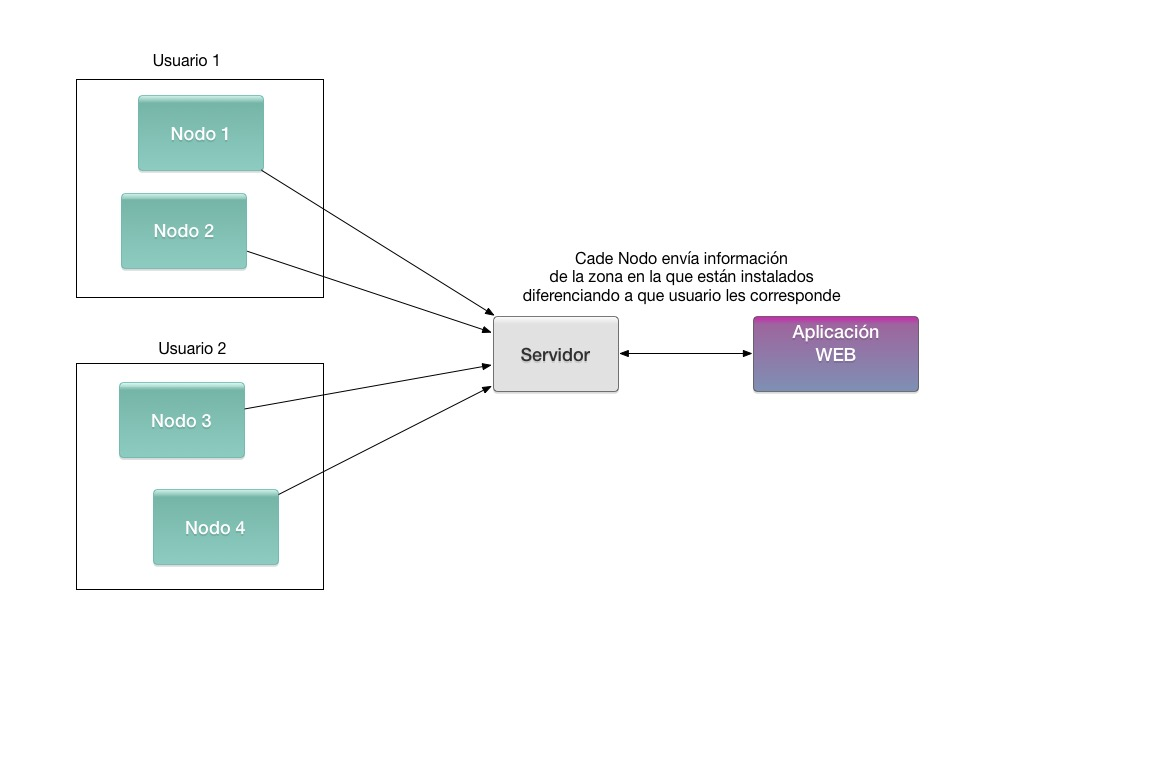
\includegraphics[width=0.9\linewidth]{figuras/montaje2}
	\caption{Esquema del funcionamiento de la aplicación}
	\label{fig:montaje2}
\end{figure}

\setlength{\parindent}{5ex}En la \textbf{Figura \ref{fig:montaje2}} se muestra el diagrama de la aplicación en el servidor en el que se dispone de una aplicación que recoge la información y la gestiona para que cada dispositivo o nodo se le pueda asignar a un usuario, este puede tener uno o muchos nodos y estos están recogiendo información independiente unos de otros y la almacena en la base de datos de manera organizada.
En la aplicación pueden haber muchos usuarios y cada uno puede almacenar la información de cada uno de sus nodos.

\clearpage

\section{Gestión de la información}

La gestión de la información es sencilla, se trata de una base de datos simple en la que se almacenará la información de los nodos, la estructura de esta base de datos esta creada automáticamente por Laravel la cual hay que especificarle el siguiente diagrama E-R:
\setlength{\parindent}{0ex}
\begin{figure}[!h]
	\centering
	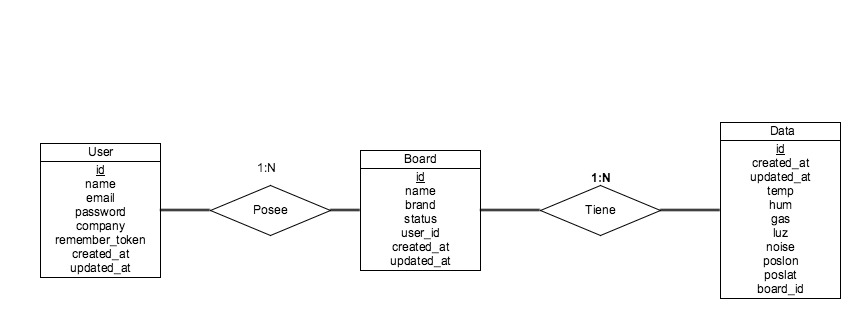
\includegraphics[width=0.9\linewidth]{figuras/diagramaer}
	\caption{Diagrama Entidad-Relación de la base de datos}
	\label{fig:bd1}
\end{figure}

Esta base de datos ha sido creada automáticamente por \textit{Artisan} de Laravel, la gestión automática crea la tabla de \textit{usuarios} y algunos campos por defecto como \textit{created\_at} y \textit{updated\_at} sin embargo el resto de los campos hay que añadirlos manualmente así como especificar los tipos de relación entre los campos, este es el código del fichero alojado en l\textit{aravel-tfg/database/migrations/tfgDatabase.php} que especifica estos campos en la BD.\\

\begin{lstlisting}[caption=Migracion de la base de datos, label=migration]
class TfgDatabase extends Migration{
	/**
	* Run the migrations.
	* @return void
	*/
	public function up(){
		Schema::create('board', function (Blueprint $table) {
			$table->increments('id');
			$table->string('name');
			$table->string('brand');
			$table->string('status');
			$table->integer('user_id')->unsigned();
			$table->timestamps();
			$table->foreign('user_id')->references('id')->on('users');
		});
		Schema::create('data', function (Blueprint $table) {
			$table->increments('id');
			$table->timestamps();
			$table->string('temp');
			$table->string('hum');
			$table->string('gas');
			$table->string('luz');
			$table->string('noise');
			$table->string('poslon');
			$table->string('poslat');
			$table->integer('board_id')->unsigned();
			$table->foreign('board_id')->references('id')->on('board');
		});
	}
	/**
	* Reverse the migrations
	* @return void
	*/
	public function down(){
		Schema::drop('data');
		Schema::drop('board');
	}
\end{lstlisting}

Si se quisieran añadir mas sensores a la aplicación se tiene que insertar  una nueva entrada en la tabla data y luego aplicar la migración como se ha visto en el  \textbf{Código \ref{phpmigrate}}.

\section{Gestión del \textit{NodeTracker}}


\setlength{\parindent}{5ex}Una vez explicado como se almacena la información se procederá como puede acceder un usuario a la aplicación la cual se ha llamado \textit{NodeTracker}, Para ello hay que o bien instalarla y configurar los nodos a la dirección del servidor o bien acceder al servidor ya instalado en la siguiente URL:
\setlength{\parindent}{0ex}
\\
\url{http://84.123.151.120:8888/}

Una vez aparecerá el Login del Nodetracker, en el cual se podrá crear un usuario o entrar con uno ya disponible:

\begin{figure}[!h]
	\centering
	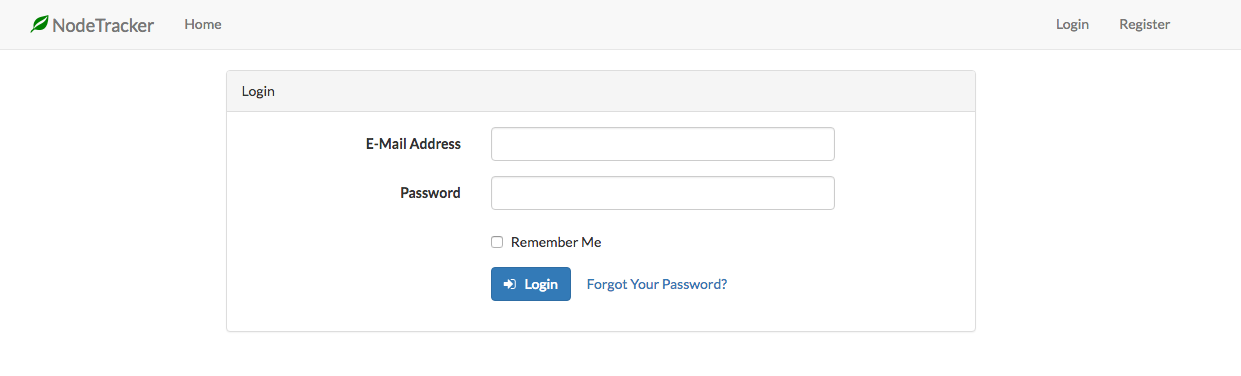
\includegraphics[width=1.0\linewidth]{figuras/loginnode}
	\caption{Login del NodeTracker}
	\label{fig:loginnode}
\end{figure}

Una vez Logueado en la aplicación se muestra lo que se ha denominado como el Home, un panel para la gestión de los diferentes nodos la cual incorporara la funcionalidad de editar el usuario o añadir nuevos nodos.

\begin{figure}[!h]
	\centering
	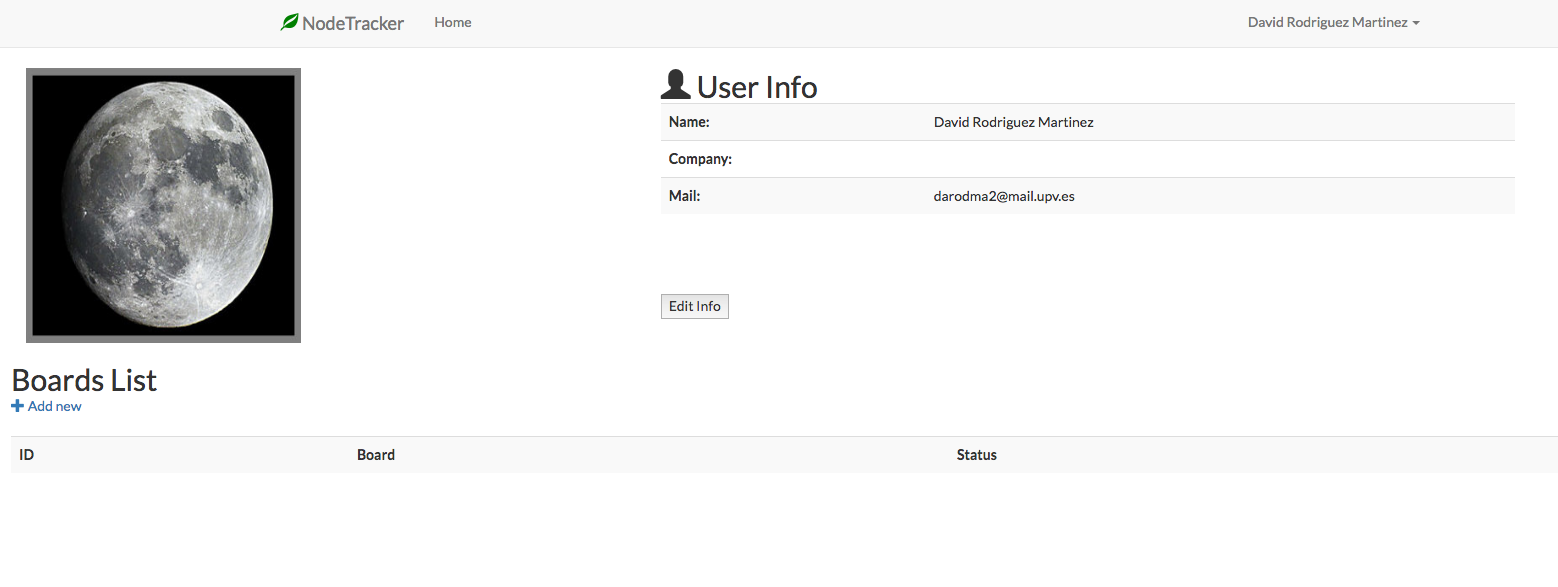
\includegraphics[width=1.0\linewidth]{figuras/homenode}
	\caption{Home del NodeTracker}
	\label{fig:homenode}
\end{figure}

Con un pequeño formulario se puede editar la información básica del usuario (\textbf{Figura \ref{fig:editusernode}}) y ademas como se había diseñado para esta aplicación se pueden añadir uno o mas nodos (\textbf{Figura \ref{fig:addnode}}), esta funcionalidad devolverá una ID en la tabla la cual se tendrá que modificar en el código del Arduino con el fin de que guarde la información correcta correspondiente al nuevo nodo en la base de datos. 

\begin{figure}[!h]
	\centering
	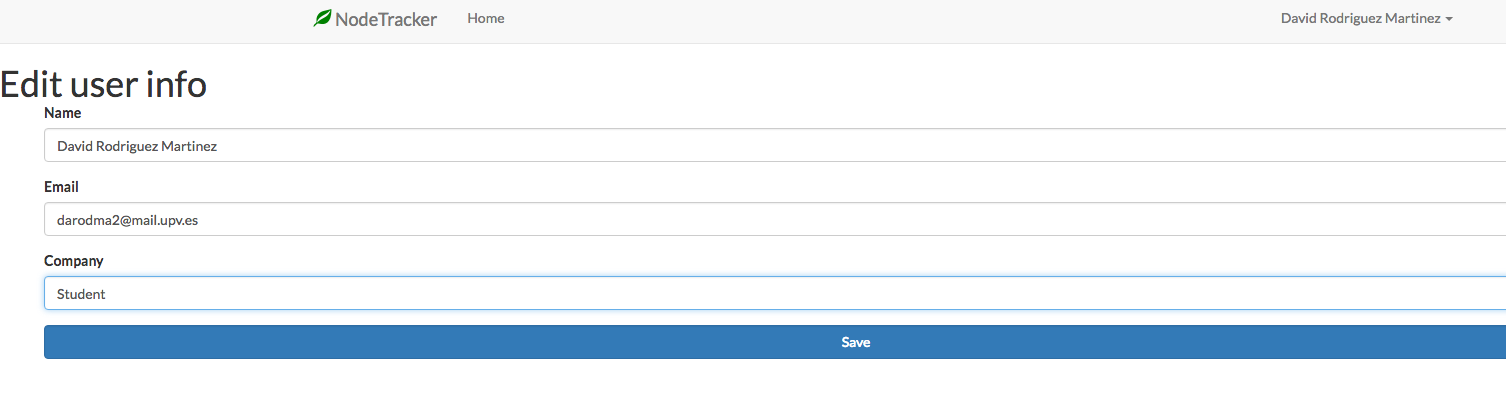
\includegraphics[width=0.7\linewidth]{figuras/edituser}
	\caption{Formulario de edición de usuarios del \textit{NodeTracker}.}
	\label{fig:editusernode}
\end{figure}

\begin{figure}[!h]
	\centering
	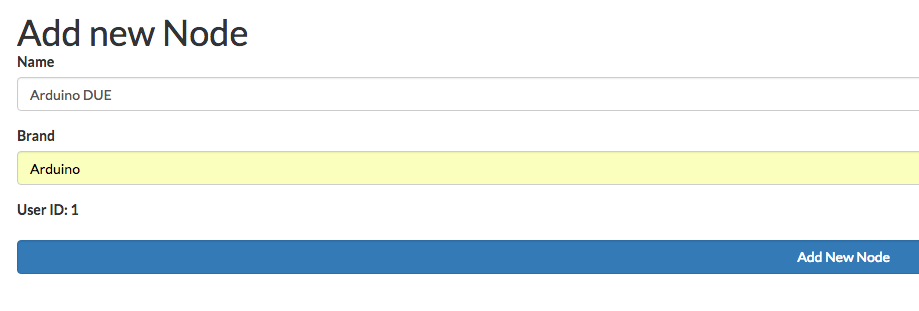
\includegraphics[width=0.7\linewidth]{figuras/addnode}
	\caption{Formulario para añadir un nuevo nodo al sistema.}
	\label{fig:addnode}
\end{figure}

Una vez creado para poder asignarlo al Arduino devolverá una ID para poder asignársela al nodo.

\begin{figure}[!h]
	\centering
	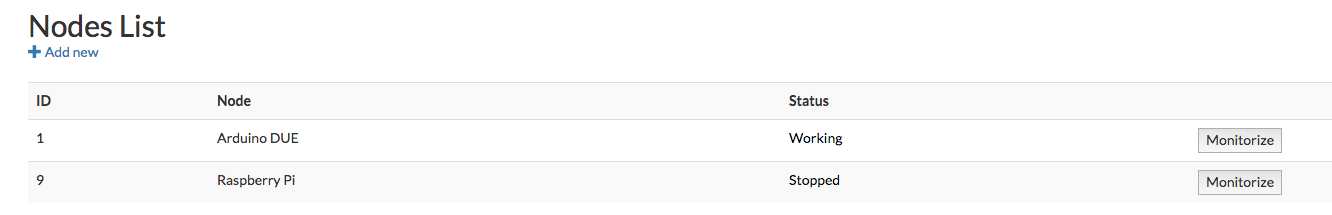
\includegraphics[width=1.0\linewidth]{figuras/nodelist}
	\caption{Lista de nodos disponibles}
	\label{fig:nodelist}
\end{figure}

En la \textbf{Figura \ref{fig:nodelist}} se puede ver la ID el nombre asignado y el estado del nodo que por defecto viene parado, para poder enlazar los nodos con la aplicación hay que visualizar la ID i añadirla en la función del código que recoge la ID en el Arduino, pero básicamente hay que cambiar en la String a enviar al servidor, por ejemplo si se quisiera enviar información desde una Raspberry Pi la cual la ID es 9, habrá que configurar la String tal que así:

\begin{lstlisting}[caption=Ejemplo para una ID diferente, label=getstringexaple]
192.168.1.16:8888/call?board_id= 8....
\end{lstlisting}

También esta el botón que redirigirá a la pagina de los reportes para poder visualizar la información obtenida que es la parte fuerte de la aplicación, es un panel donde se podrá visualizar la información o generar un reporte con la información recogida.
\clearpage

\section{Visualización  de la información}

\begin{figure}[!h]
	\centering
	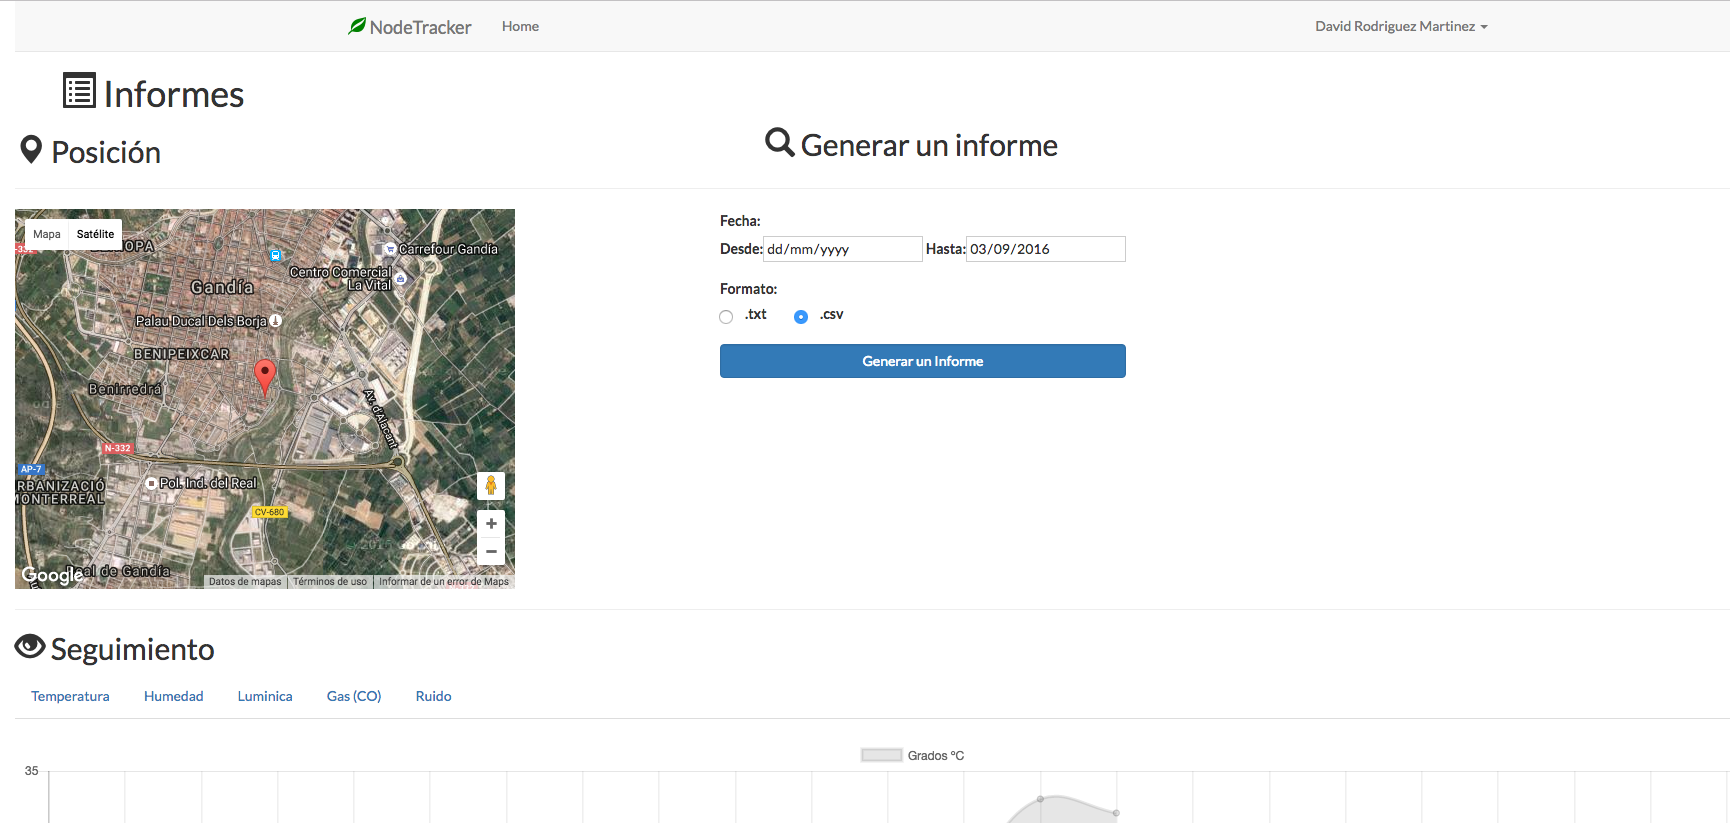
\includegraphics[width=1.0\linewidth]{figuras/nodereport}
	\caption{Pagina de monitorización de la aplicación}
	\label{fig:nodereport}
\end{figure}

Esta es la pagina en la cual se podrá visualizar la informacion, consta de 3 secciones, un mapa para mostrar la ubicación de la ultima entrada a la base de datos, otra sección que se encargara de generar los reportes para poder trabajar con ellos, y una gráfica que intentara mostrar un progreso de la informacion recogida a lo largo del día.

\subsection{Posicionamiento}

Para ello esta el Mapa en la seccion de \textit{Position} que gracias a la API de Google MAPS se ha podido implementar esta funcionalidad, en este caso el mapa es en vista satélite ya que al ser una aplicación medioambiental, se necesitara saber si el nodo esta en un núcleo urbano o en territorio natural, y aproximadamente a que altura se puede encontrar, costa o altas montañas. \textit{Para el ejemplo de la \textbf{Figura \ref{fig:nodereport}} se dispone de las coordenadas -0.180812 y 38.960541 que corresponden al termino municipal de Gandia.} 

\subsection{Obtener un informe}

Se ha implementado una función para generar informes, llamada \textit{Reports} la cual generará un informe definido por un rango de fechas.

\begin{figure}[!h]
	\centering
	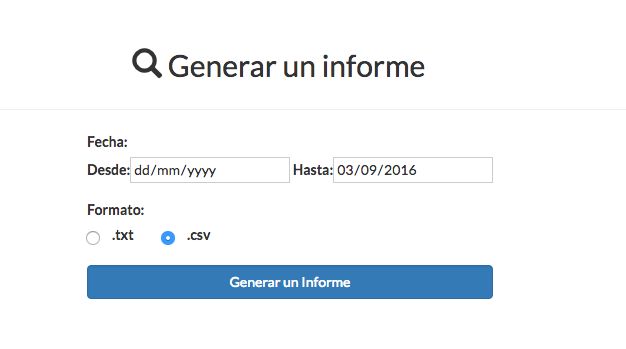
\includegraphics[width=0.8\linewidth]{figuras/nodereports2}
	\caption{Generación de Informes}
	\label{fig:nodereport}
\end{figure}

Esta función generara un informe en formato JSON de la informacion recogida cada minuto por el nodo unido a la aplicación, el resultado puede variar en el formato escogido en este caso .txt (texto plano) o .csv (Hojas de calculo para LibreOfice) para poder trabajarlas en otras aplicaciones o realizar migraciones de estas, muy útil para la minería de datos que, utilizando programas en R o Python se puede trabajar este formato JSON.

\subsection{Seguimiento de la informacion}

Por ultimo el la función de monitorización, llamada \textit{monitoring} se ha implementado una gráfica utilizando la API de Chart.js que permitirá realizar un seguimiento los valores recogidos en cada hora de ese mismo día realizando un promedio de los valores obtenidos en esa hora del día, ya que implementar cada minuto seria visualmente cargado y podría desestabilizar la gráfica si se presentan valores anómalos. 
Ademas presenta una gráfica diferente para cada valor a medir (temperatura, humedad, gases, luz y ruido) que implementado con AJAX realiza el cambio de gráfica sin necesidad de refrescar la pagina.

\begin{figure}[!h]
	\centering
	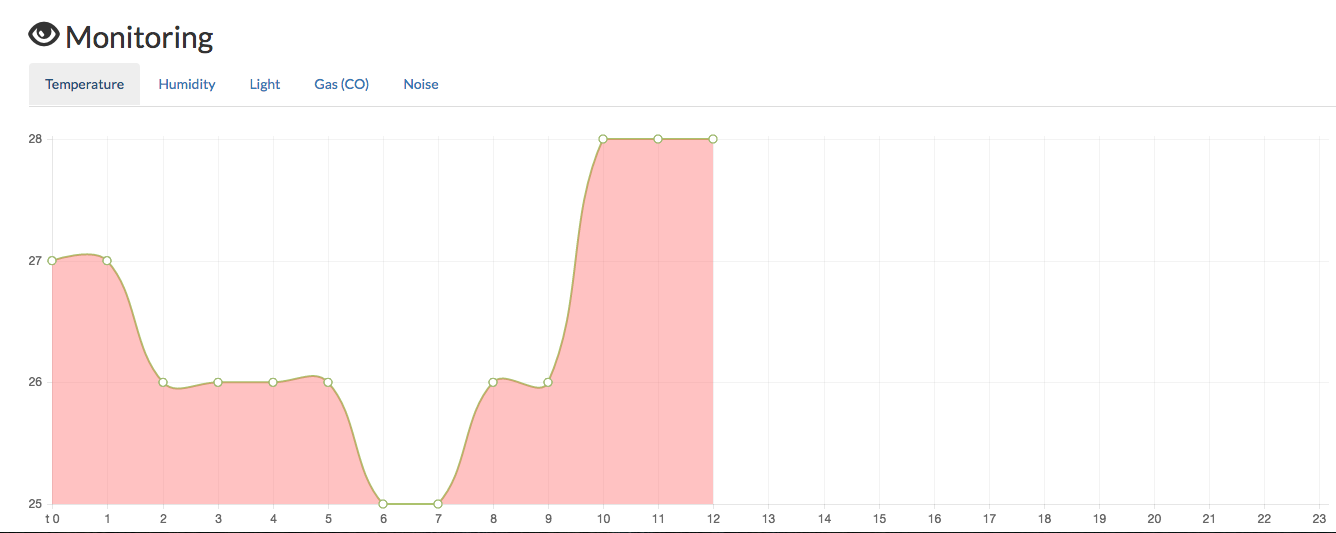
\includegraphics[width=0.9\linewidth]{figuras/nodereports3}
	\caption{Grafica perteneciente a la temperatura en el seguimiento}
	\label{fig:nodereport}
\end{figure}






%%%%%%%%%%%%%%%%%%%%%%%%%%%%%%%%%%%%%%%%%%%%%%%%%%%%%%%%%%%%%%%%%%%%%%%%%%%%%%%
%                                 CONCLUSIONS                                 %
%%%%%%%%%%%%%%%%%%%%%%%%%%%%%%%%%%%%%%%%%%%%%%%%%%%%%%%%%%%%%%%%%%%%%%%%%%%%%%%


\chapter{Conclusiones y mejoras}

\section{Seguridad}

\setlength{\parindent}{5ex}Después de Utilizar Arduino he podido apreciar que es bastante bueno para el aprendizaje pero para una aplicación real deja mucho que desear ya que en un entorno educacional si se produce algún error se puede corregir en el momento y estos no serán provocados, ademas debido a la incapacidad nativa del SAM3X para encirptar la informacion, en este caso pretendía realizar peticiones HTTPS al servidor, el sistema es muy debil a ataques MitM (\textit{Man-in-the-middle}) pues la informacion que envía no esta encirptada de ningún modo ni existe algún tipo de bloqueo a peticiones externas que no tengan nada que ver con la aplicación por lo que esto queda muy lejos de ser una aplicación final pues se puede romper por este hueco de seguridad.

\setlength{\parindent}{0ex}\textit{Un ataque man-in-the-middle es un ataque en el que se adquiere la capacidad de leer, insertar y modificar a voluntad, los mensajes entre dos partes sin que ninguna de ellas conozca que el enlace entre ellos ha sido violado. El atacante debe ser capaz de observar e interceptar mensajes entre las dos víctimas.}\cite{mitm}.

Para solucionar esto, he pensado en utilizar controladoras que permitan encriptación o conexión SSH lo cual requeriría un rendimiento mayor y un mayor consumo, o también, la aplicación solo pueda estar disponible para una red interna, lo que la limitaría a un área muy reducida ya que si esta conectada a Internet, el área de alcance es a nivel global pero insegura, por lo que resolviendo algunos problemas surgen otros nuevos.

\section{Sensores}

\setlength{\parindent}{5ex}He tenido aprendizaje en el funcionamiento de la electrónica básica ha sido gracias a los diversos problemas entre versiones de Arduino y los cambios realizados en los circuitos para poder implementarlos.
\setlength{\parindent}{0ex}
Ademas de otros problemas, los sensores no dan siempre un valor fiable, en el proyecto los he tratado como valores anómalos, los cuales son valores que no corresponden con lo que deberían de dar ya sea por error de lectura o fallo de los componentes debido a su montaje en cableado.

Para poder solucionar esto habría que tener en cuenta 2 casos:

\begin{itemize}
	\item \textbf{Circuito:} Todo esto podría mejorar si en vez de implementa el circuito en una \textit{protoboard} se habría creado un circuito impreso y soldado los componentes directamente a la placa y estos pines conectarlos al Arduino con el fin de suprimir la \textit{protoboard}, cables y componentes de electrónica básica que permiten funcionar correctamente los sensores. Esto suprimiría los errores de fallos de conexión o cortocircuitos en la aplicación ademas de reducir notablemente el tamaño del nodo.   
	
	\item \textbf{Sensores} Los sensores que he utilizado para el proyecto son de un coste reducido, por ejemplo, hay sensores que durante el montaje de este proyecto se han quemado, no son para una larga duración, debido a su coste y tampoco son muy exactos, para solucionar esto se deberían implementar sensores mas eficientes de un coste mas elevado, por ejemplo reemplazar el DHT11 de unos 2\euro por su versión mas cara el DHT33 por 17\euro.

\end{itemize}

\section{Boards especializadas}

\setlength{\parindent}{5ex}Analizando en este proyecto lo que he podido obtener de informacion sobre Arduino es que no sirve mucho para realizar este tipo de funciones, como se ha descrito anteriormente solo sirve para el ámbito educacional y demás, sin embargo todo este sistema ya existe a nivel comercial, así que analizando en Internet he obtenido informacion sobre una controladora que, ofrezca la informacion segura y que permita conectarse por una red, tanto cableada como inalámbrica (incluyendo GPRS) y que tenga un consumo muy reducido.
\setlength{\parindent}{0ex}
Se trata de la controladora FlyPort que en cierta medida soluciona los problemas que se han descrito anteriormente sin embargo lejos de ser la panacea el problema es que al ser comercial su precio es muy elevado ya que aunque la controladora sea barata, requiere de un sistema para poder implementar los sensores y poder programarla.

En la \textbf{Figura \ref{fig:flyportimg}} esta la imagen del \textit{Started kit} de la controladora en cuestión: 

\begin{figure}[!h]
	\centering
	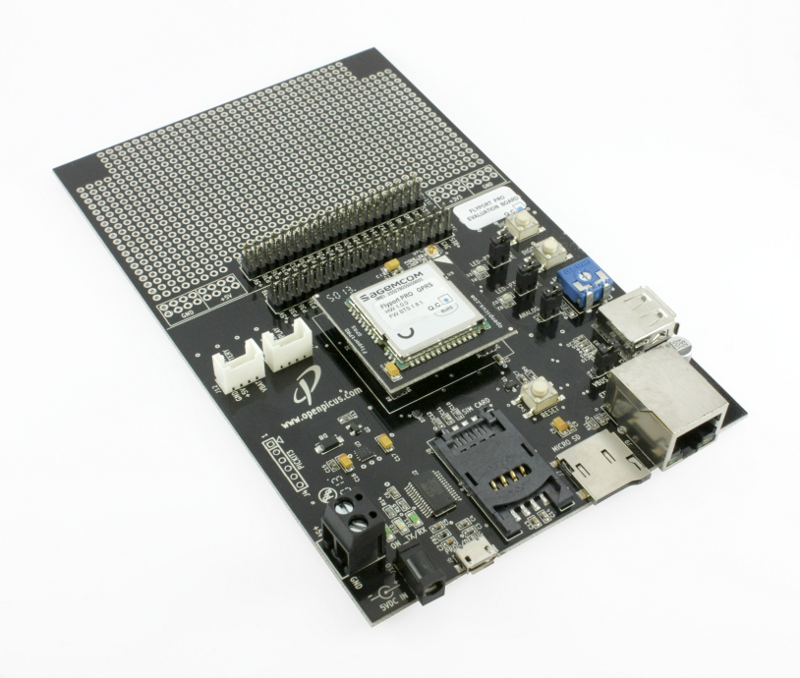
\includegraphics[width=0.5\linewidth]{figuras/flyportimg}
	\caption{FlyPort GPRS y la placa para la controladora.\cite{FlyPort}}
	\label{fig:flyportimg}
\end{figure}

El coste de este \textit{Started kit} es de unos 150\euro aproximadamente y como he hablado en la sección anterior también se va a añadir el coste de sensores de calidad al nodo, teniendo en cuenta que al ser de calidad son de un coste mucho mas caro que los que he utilizado para este proyecto, el coste puede subir perfectamente a los 200\euro




%%%%%%%%%%%%%%%%%%%%%%%%%%%%%%%%%%%%%%%%%%%%%%%%%%%%%%%%%%%%%%%%%%%%%%%%%%%%%%%
%                                BIBLIOGRAFIA                                 %
%%%%%%%%%%%%%%%%%%%%%%%%%%%%%%%%%%%%%%%%%%%%%%%%%%%%%%%%%%%%%%%%%%%%%%%%%%%%%%%

\begin{thebibliography}{10}

%%%%%%%%%%%%%%%%%%%%%%%%%%%%%%%%%%%%%%%%%%%%%%%%%%%%%%%%%%%%%%%%%%%%%%%%%%%%%%%
% MODEL D'ARTICLE                                                             %
%%%%%%%%%%%%%%%%%%%%%%%%%%%%%%%%%%%%%%%%%%%%%%%%%%%%%%%%%%%%%%%%%%%%%%%%%%%%%%%
%\bibitem{light}
%Jennifer~S. Light.
%\newblock When computers were women.
%\newblock \textit{Technology and Culture}, 40:3:455--483, juliol, 1999.

%%%%%%%%%%%%%%%%%%%%%%%%%%%%%%%%%%%%%%%%%%%%%%%%%%%%%%%%%%%%%%%%%%%%%%%%%%%%%%%
% MODEL DE LLIBRE                                                             %
%%%%%%%%%%%%%%%%%%%%%%%%%%%%%%%%%%%%%%%%%%%%%%%%%%%%%%%%%%%%%%%%%%%%%%%%%%%%%%%
%\bibitem{ifrah}
%Georges Ifrah.
%\newblock \textit{Historia universal de las cifras}.
%\newblock Espasa Calpe, S.A., Madrid, sisena edició, 2008.

%%%%%%%%%%%%%%%%%%%%%%%%%%%%%%%%%%%%%%%%%%%%%%%%%%%%%%%%%%%%%%%%%%%%%%%%%%%%%%%
% MODEL D'URL                                                                 %
%%%%%%%%%%%%%%%%%%%%%%%%%%%%%%%%%%%%%%%%%%%%%%%%%%%%%%%%%%%%%%%%%%%%%%%%%%%%%%%
\bibitem{Arduino}
Información sobre la redacción del TFG
\newblock consultado en 
\url{https://riunet.upv.es/}.

\bibitem{Arduino}
Información sobre Arduino DUE, conexiones y funcionamiento
\newblock consultado en 
\url{https://www.arduino.cc/en/Main/ArduinoBoardDue}.

\bibitem{NEO6mv2}
Información, decodificación, programación y DataSheet del dispositivo de Localización NEO6mv2 utilizado en el proyecto
\newblock consultado en \\
\url{https://www.u-blox.com/sites/default/files/products/documents/NEO-6_DataSheet_(GPS.G6-HW-09005).pdf}.\\
\url{http://www.gpsinformation.org/dale/nmea.htm}.\\
\url{http://arduiniana.org/libraries/tinygps/}

\bibitem{DHT11}
Información del funcionamiento y librerías del sensor DHT11
\newblock consultado en 
\url{http://playground.arduino.cc/Main/DHT11Lib}.\\
\url{https://cdn-learn.adafruit.com/downloads/pdf/dht.pdf}.

\bibitem{Parallax Gas CO sensor}
Información del funcionamiento y DataSheet del sensor Parallax Gas CO sensor MQ-7
\newblock consultado en 
\url{https://www.parallax.com/sites/default/files/downloads/27904-Gas-Sensor-Modules-Guide-v2.3.pdf}.

\bibitem{Laravel 5.2}
Información sobre como desarrollar una aplicación WEB utilizando el Framework Laravel 5.2
\newblock consultado en 
\url{https://laravel.com/docs/5.2}.


\end{thebibliography}

\cleardoublepage

%%%%%%%%%%%%%%%%%%%%%%%%%%%%%%%%%%%%%%%%%%%%%%%%%%%%%%%%%%%%%%%%%%%%%%%%%%%%%%%
%                           APÈNDIXS  (Si n'hi ha!)                           %
%%%%%%%%%%%%%%%%%%%%%%%%%%%%%%%%%%%%%%%%%%%%%%%%%%%%%%%%%%%%%%%%%%%%%%%%%%%%%%%

\APPENDIX

%%%%%%%%%%%%%%%%%%%%%%%%%%%%%%%%%%%%%%%%%%%%%%%%%%%%%%%%%%%%%%%%%%%%%%%%%%%%%%%
%                         LA CONFIGURACIO DEL SISTEMA                         %
%%%%%%%%%%%%%%%%%%%%%%%%%%%%%%%%%%%%%%%%%%%%%%%%%%%%%%%%%%%%%%%%%%%%%%%%%%%%%%%


%%%%%%%%%%%%%%%%%%%%%%%%%%%%%%%%%%%%%%%%%%%%%%%%%%%%%%%%%%%%%%%%%%%%%%%%%%%%%%%
%                               ALTRES  APÈNDIXS                              %
%%%%%%%%%%%%%%%%%%%%%%%%%%%%%%%%%%%%%%%%%%%%%%%%%%%%%%%%%%%%%%%%%%%%%%%%%%%%%%%


%%%%%%%%%%%%%%%%%%%%%%%%%%%%%%%%%%%%%%%%%%%%%%%%%%%%%%%%%%%%%%%%%%%%%%%%%%%%%%%
%                              FI DEL DOCUMENT                                %
%%%%%%%%%%%%%%%%%%%%%%%%%%%%%%%%%%%%%%%%%%%%%%%%%%%%%%%%%%%%%%%%%%%%%%%%%%%%%%%

\end{document}
